 \documentclass{report}
 
\usepackage[utf8]{inputenc} 
\usepackage[T1]{fontenc}      
\usepackage[top=3.5cm, bottom=3cm, left=3.0cm, right=4.0cm]{geometry}
\usepackage{graphicx}
\graphicspath{{figures/}{../figures}}

\begin{document}

\section*{Question de cours}
Énoncez le premier principe de la thermodynamique. A quelle loi fondamentale de la physique se réfère t-il ?

\section*{Exercice 1}

\subsection*{Machine 1}

On considère le cycle ci-dessous décrit par une mole de gaz parfait. Les transformations $A\rightarrow B$ et $C\rightarrow D$ sont des adiabatiques réversibles. On supposera que $\gamma$ est constant.

\begin{itemize}
	\item[•] A quel type de machine a t-on affaire ? Décrivez chaque transformation.
	\item[•] Calculez son rendement en fonction de $a$ et $\gamma$.
	%\item[•] Comparez le rendement de ce moteur avec celui d'un moteur décrivant un cycle de Carnot. Commentez. 
\end{itemize}

\textit{Données : $ V_{2}/V{1} = 10$ et $ \gamma=1.4$}

\begin{figure}[!h]
\centering
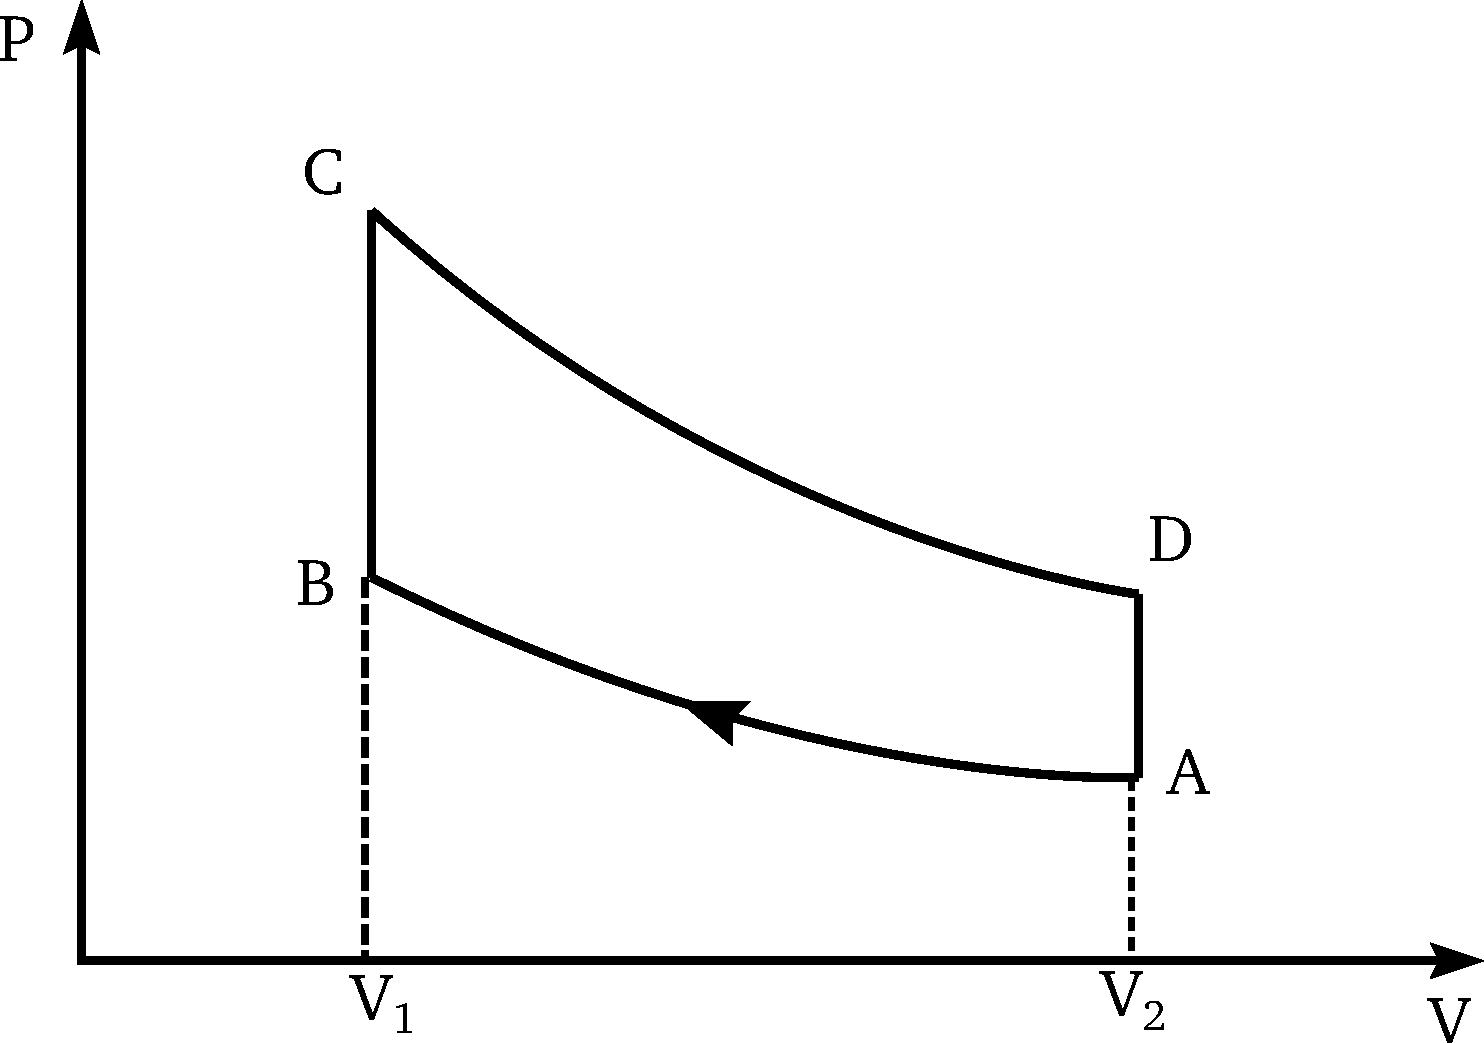
\includegraphics[width=0.3\linewidth]{cycle_beau_rochas.pdf}
\end{figure}

\subsection*{Machine 2}

L'air enfermé dans un cylindre de volume $V=1L$ subit la suite de transformations réversibles suivantes :
\begin{itemize}
\item[•]$A \rightarrow B$ : isotherme
\item[•]$B \rightarrow C$ : adiabatique
\item[•]$C \rightarrow D$ : isotherme
\item[•]$D \rightarrow A$ : adiabatique

\end{itemize}
On donne : $P_{A}=1$ bar, $V_{A} = 1L$, $T_{A}=300K$, $ P_{C}=50$ bar, $V_{B} = V_{A}/8$, $\gamma=1.4$

\begin{itemize}
\item[•] Calculez le travail fourni par le gaz sur le piston au cours d'un cycle et la chaleur fournie par la source chaude sur un cycle.
\item[•] Calculez le rendement, et comparer avec le rendement théorique.
\item[•] Calculez la puissance du moteur sachant que le fluide effectue 5000 cycles par minute. 
\end{itemize}

\newpage

\section*{Exercice 2}

On étudie l'écoulement d'un gaz dans une tuyère horizontale isolée thermiquement du milieu extérieur.

En régime permanent, dans une section droite de la tuyère les vitesses d'écoulement sont égales et normales à la section. La pression et la température sont indépendantes du temps et uniformes :
\begin{itemize}
\item[-]à l'entrée de la tuyère, $x=x_{1}$ : $P_{1} = 3$ bars; $T_{1} = 300$ K;
\item[-]à la sortie de la tuyère, $x=x_{2}$ : $P_{2} = 1$ bars; $T_{2} = 250$ K
\end{itemize}

Soit $H_{m}(x)$ l'enthalpie molaire du gaz à l'abscisse $x$ et $M$ la masse molaire du gaz. 

\begin{itemize}
\item[•] Montrer que pour une mole de gaz passant dans la tuyère, on peut écrire $H_{m}(x)+\frac{1}{2}Mv^{2}(x)= cste$.
\item[•] On suppose que $v(x_{1})$ négligeable, calculer $v(x_{2})$. On supposera le gaz parfait. 
\end{itemize}

\textit{Données : $M = 32g.mol^{-1}$ et $\gamma=1.4$}

\begin{figure}[!h]
\centering
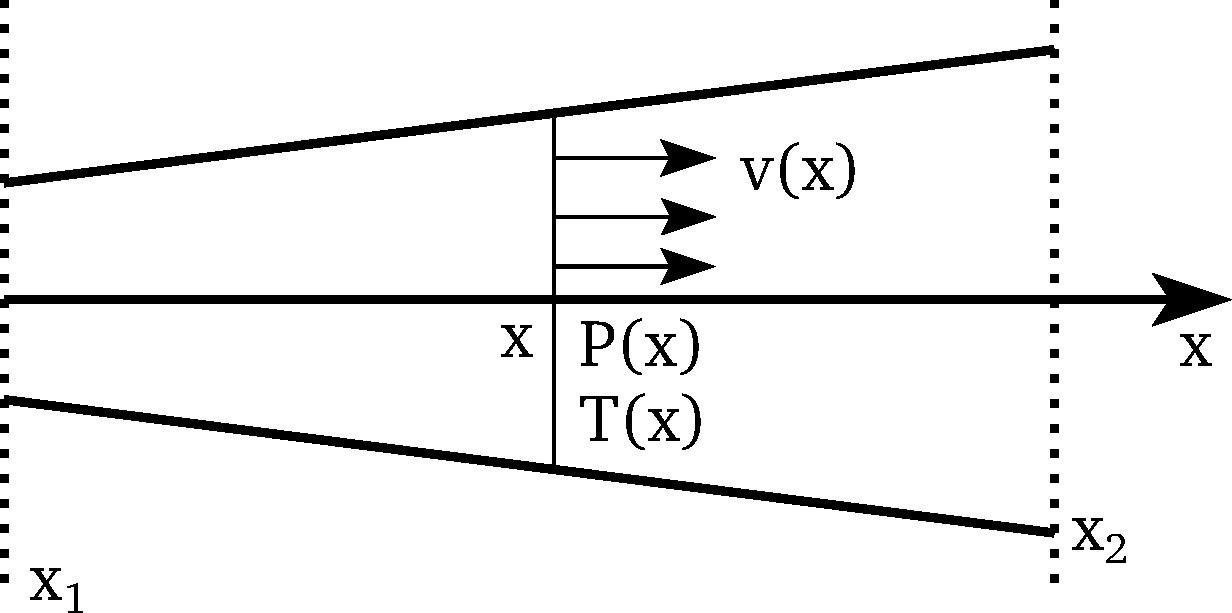
\includegraphics[width=0.4\linewidth]{turbine.pdf}
\end{figure}

\subsubsection*{Étude d'une turbine}
On suppose que le gaz est utilisé à la sortie pour actionner une turbine située dans la tuyère. A l'entrée, il a une vitesse $v_{2}$, une température $T_{2}$ et une pression $P_{2}$. A la sortie, la pression et la température sont inchangées, mais la vitesse est nulle. 
\begin{itemize}
\item[•] Calculer le travail récupéré par la turbine lors du passage d'une mole de gaz.

\end{itemize}

\subsubsection*{Étude d'une fusée}

On suppose désormais que la tuyère est celle d'un propulseur spatial, équipant une fusée de masse $M_0$ à vide, contenant une masse $m_0$ de gaz carburant. Le gaz est stocké sous pression à une température initiale $T_1$ et est éjecté à une température $T_2$. On négligera les différences entre le cas où la tuyère est horizontale ou verticale et toute force de frottement sur la fusée. 

\begin{itemize}
	\item[•] Comment relier la vitesse d'éjection des gaz $v_2$ avec la variation de la vitesse $\frac{d}{dt} V(t)$ de la fusée ? 
	\item[•] Quelle est la vitesse de la fusée lorsque tout le gaz a été éjecté ?
\end{itemize}

\newpage

\section*{Exercice 3}

\subsection*{Premier principe}

Une ampoule de volume de $V_1$, dans laquelle règne le vide, est entourée d'air ambiant à la pression $P_{0} = 1$atm et à la température $T_{0}=20^{\circ}C$, qu'on assimile à un gaz parfait de coefficient $\gamma=1.4$. On perce un petit trou dans l'ampoule, l'air s'y engouffre et au bout d'une durée très courte, la pression dans l'ampoule est égale à la pression ambiante.

Quel est la température $T_{1}$ dans l'ampoule une fois celle-ci remplie?

\begin{figure}[!h]
\centering
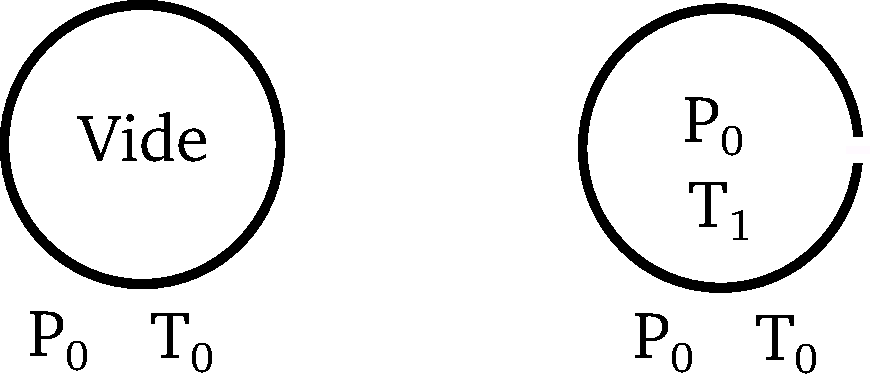
\includegraphics[width=0.5\linewidth]{ampoule.pdf}
\end{figure}

\section*{Second principe}

Soit un système de volume constant constitué d'un nombre $N>>1$ de particules en équilibre à la température T et dont chacune peut avoir deux niveau d'énergie $E_{1}$ et $E_{2}$, avec $E_{1}<E_{2}$.

Soit $n_{1}$ le nombre de particules dans l'état d'énergie $E_{1}$ et $n_{2}$ le nombre de particules dans l'état d'énergie $E_{2}$.

On suppose que la répartition des particules se fait selon la loi de Boltzmann :
\begin{equation}
\frac{n_{2}}{n_{1}}=exp\left( \frac{E_{2}-E_{1}}{k_{b}T}\right) 
\end{equation}

Cette distribution indique que les niveaux ont d'autant plus de chance d'être peuplés qu'ils n'ont pas une énergie élevée. D'autre part plus la température est élevée, plus les niveaux d'énergies élevées pourront être peuplés. 

\begin{itemize}
\item[-]Déterminez la différentielle de l'énergie interne du système en fonction de $n_{1}$ et $E_{2}-E_{1}$.
\item[-]On rappelle que l'entropie peut s'écrire comme $S=k_B\log\Omega$, où $\Omega$ est le nombre de configurations possibles pour le système.. Exprimez $S$ en fonction de $N$ et $n_1$. On utilisera la formule de Stirling $\ln (N!)=N \ln (N)$ valable pour $N>>1$.
\item[-] Exprimez la différentielle de $S$ en fonction de $T$, $\Delta$ et $n_1$.
\item[-] Montrez que l'on retrouve l'identité thermodynamique : $dU = TdS$
\end{itemize}

\newpage

\section*{Question de cours}
Énoncez et démontrez l’inégalité de Clausius.

\section*{Exercice 4}

Dans tout le problème, les échanges de travail et de chaleur seront toujours considérés du point de vue du gaz.
\begin{itemize}

\item[•] On considère le réfrigérant représenté ci-dessous, qu'on suppose parfaitement calorifugé. Le gaz, de chaleur massique $c_{p}$ est refroidi à pression constante, de la température $T_{2}$ à la température $T_{3}$, au moyen d'un circuit d'eau (de chaleur massique $c$ constante), qui, elle, est réchauffée de $t_{0}$ à $t_{1}$.

\begin{figure}[!h]
\centering
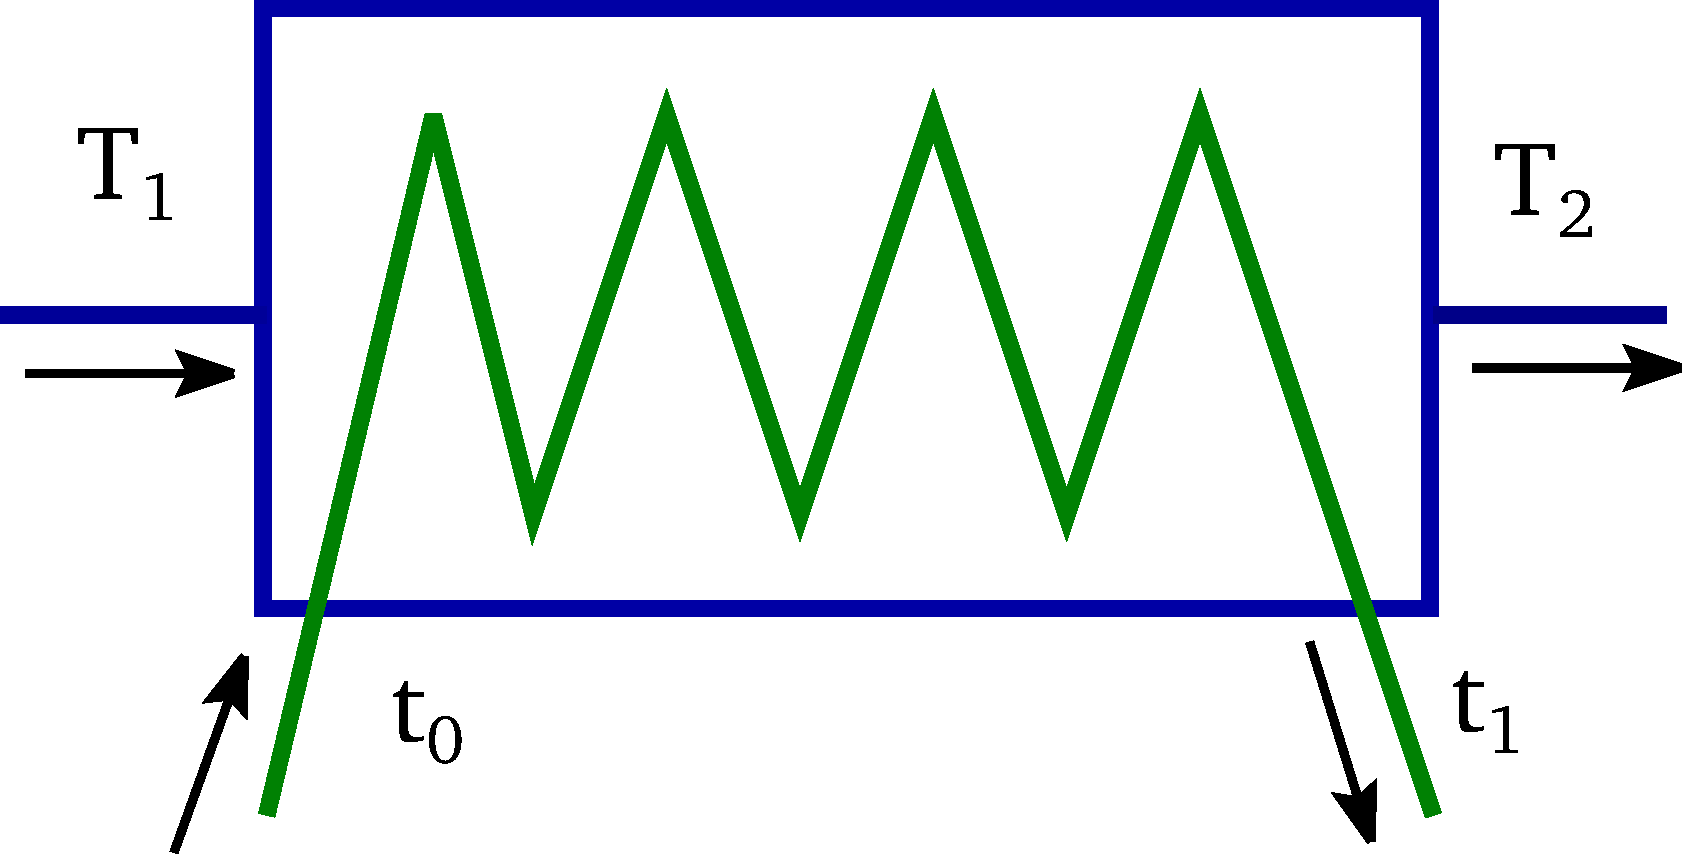
\includegraphics[width=0.3\linewidth]{refrigirant.pdf}
\end{figure}

Le débit massique du gaz étant imposé, déterminer le débit massique $D$ nécessaire du circuit d'eau de refroidissement.
\item[•] On considère maintenant un échangeur de chaleur représenté ci-dessous. Il comporte deux canalisations dans lesquelles le même gaz circule avec le même débit mais dans des sens opposés. Les températures d'entrées, supposées connues, seront notées $T_{4}$ et $T_{9}$ et les température de sorties respectives $T_{5}$ et $T_{10}$. Dans chaque canalisation, la pression est constante.
\begin{figure}[!h]
\centering
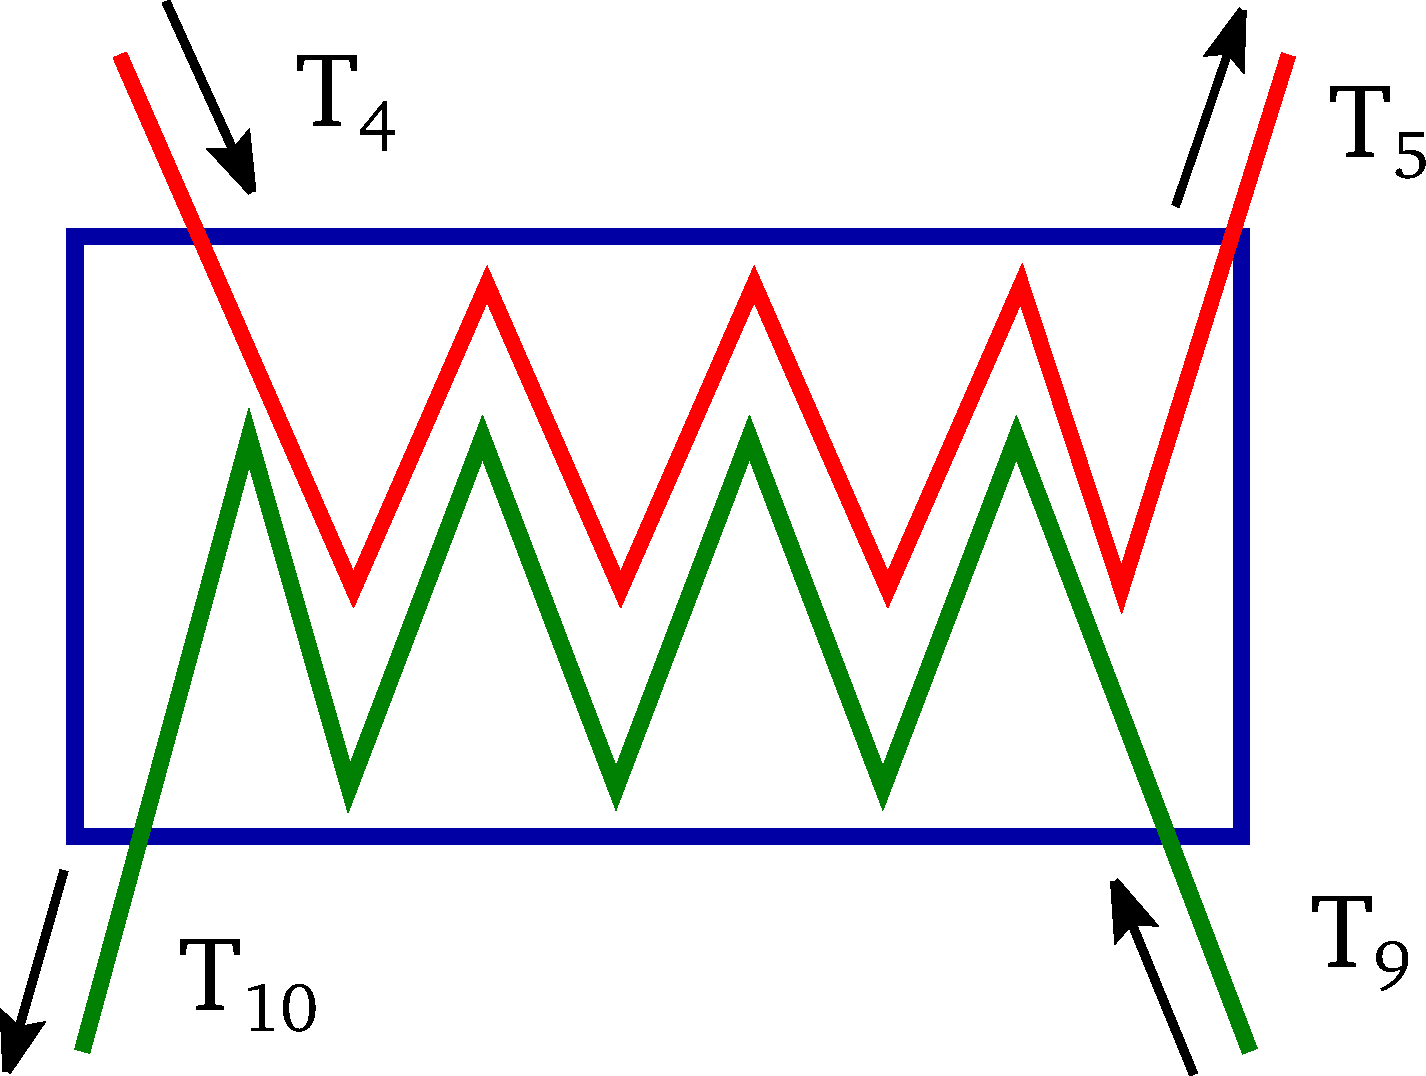
\includegraphics[width=0.3\linewidth]{echangeur.pdf}
\end{figure}
On suppose d'abord réversible les transformations subies par le gaz dans chaque canalisation. En utilisant les fonctions enthalpie et entropie, écrire les relations reliant $T_{5}$ et $T_{10}$ à $T_{4}$ et $T_{9}$.

En déduire les solutions physiquement acceptables pour $T_{5}$ et $T_{10}$.

Si les transformations sont en fait irréversibles, quel les inégalités satisfaites par $T_{5}$ et $T_{10}$, si l'on suppose $T_{4}>T_{9}$ ?

\item[•] On définit l'efficacité comme étant : $e=\frac{T_{5}-T{4}}{T_{9}-T{4}}$ en considérant la canalisation 4-5. Montrer qu'on obtient la même efficacité en considérant la canalisation 9-10.
\end{itemize}

\newpage

\section*{Exercice 5}

\begin{figure}[!h]
\centering
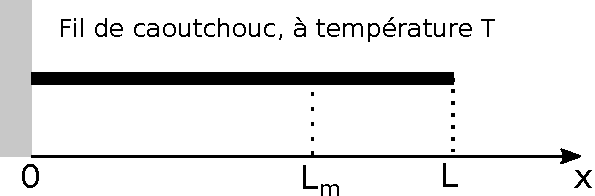
\includegraphics[width=0.4\linewidth]{thermo2.pdf}
\end{figure}

On considère un fil de caoutchouc décrit par les variables d'état : sa longueur $L$, sa température $T$ et $F$ la force appliquée dessus. Son équation d'état est de la forme : 
\begin{equation}
	F(L,T) = F_0 + \rho(L-L_0) + \sigma(T-T_0)
\end{equation}
$\rho$ et $\sigma$ sont des constantes. 

L'énergie interne du fil peut alors s'écrire : 
\begin{equation}
	U(L,T) = C_L(T-T_0)+(F_0-\sigma T_0)(L-L_0) +\frac{ \rho}{2}(L-L_0)^2 +U_0
\end{equation}
où $C_L$ est une constante. 

On attache désormais le fil de caoutchouc en $CM$, où le cercle de centre $O$ et de rayon $OM=R$ tourne à la vitesse angulaire $\omega$. On a $CO=a\ll R$. Le cercle est plongé à son diamètre entre deux source de chaleurs à températures $T_1$ et $T_2$  (avec $T_1>T_2$) :

\begin{figure}[!h]
\centering
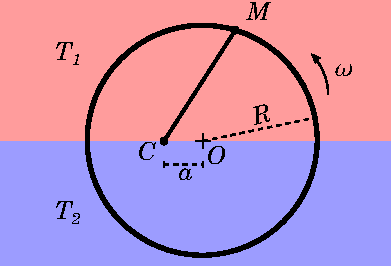
\includegraphics[width=0.3\linewidth]{thermo3.pdf}
\end{figure}

Le fil subit les transformations successives suivantes :
\begin{itemize}
\item[1 -] Une transformation isotherme à $T_1$ lorsque le fil est dans la demi-partie supérieure (rouge)
\item[2 -] Lorsque le fil passe à l'horizontale (longueur $R-a$), il passe instantanément de $T_1$ à $T_2$
\item[3 -] Une transformation isotherme à $T_2$ lorsque le fil est dans la demi-partie inférieure (bleue)
\item[4 -] Lorsque le fil passe à l'horizontale (longueur $R+a$), il passe instantanément de $T_2$ à $T_1$
\end{itemize}
Questions : 
\begin{itemize}
\item[•] Comment s'écrit le travail reçu par le fil ?
\item[•] Décrire le cycle dans un diagramme de Clapeyron.
\item[•] Calculer les divers échanges mécaniques et thermiques au cours de ce cycle.
\item[•] Le cycle proposé est-il moteur ?
\end{itemize}

\newpage

\section*{Exercice 6}

On considère un cylindre rempli d'un gaz parfait à la température $T_1$, à la pression $P_1$ et un volume $V_1=aS$, où $a$ est la hauteur et S la section.

Le cylindre est surmonté d'un piston, de masse $m$, libre de coulisser sans frottement. La pression à l'extérieur du dispositif est $P_0$.

Les parois du cylindre et du piston sont considérées comme athermane : il n'y a aucun échange thermique avec l'extérieur.

A un certain moment, on fait tomber une masse $M$ sur le piston d'une hauteur $H$. Après quelques oscillations, le piston retourne à un nouvel équilibre.


\begin{figure}[!h]
\centering
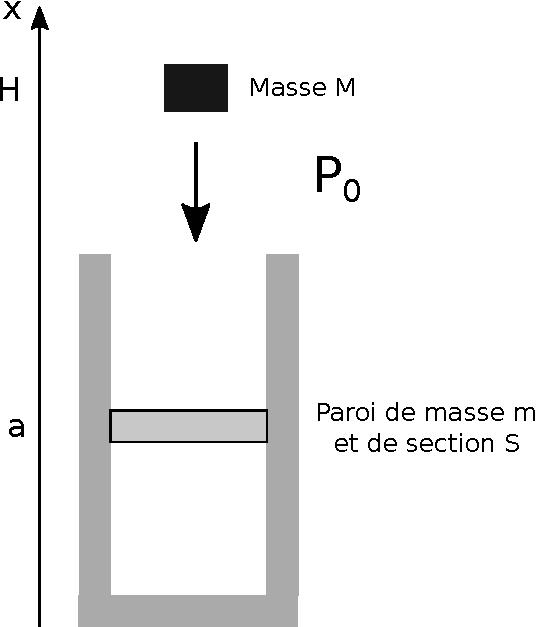
\includegraphics[width=0.5\linewidth]{thermo4.pdf}
\end{figure}

\begin{itemize}
\item[•] Calculez les paramètres internes du gaz au nouvel équilibre. 
\item[•] Pour quelle hauteur de chute $H_C$ le piston se retrouve t-il exactement à la même hauteur initiale $a$ ?
\item[•] Que se passe t-il si $M$ devient très lourde ?
\end{itemize}

\newpage

\section*{Exercice 7}

On considère le dispositif ci-dessous. Le piston (gris, entouré de noir) et les parois (en gris) sont adiabatiques. La paroi interne séparant les espaces $A$ et $B$ est fixe et diatherme. Elle est percée d'un trou fermé par une fenêtre amovible. La pression extérieure est $P_0=1$ bar. Initialement, le volume $B$ est rempli d'une mole de gaz parfait $\gamma=1,4$, avec une pression $P_0=1$ bar, une température $T_0=300$K. Le volume $A$ est vide.

\begin{figure}[!h]
\centering
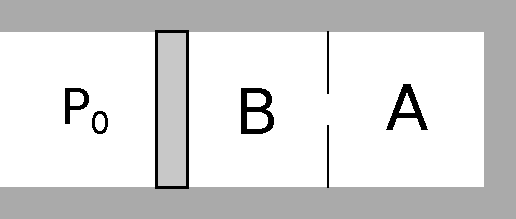
\includegraphics[width=0.5\linewidth]{thermo1.pdf}
\end{figure}

\begin{itemize}
\item[•] On ouvre la fenêtre. Décrire qualitativement ce qu'il se passe suivant le volume de $A$. En déduire l'existence d'un volume critique $V_C$ que l'on ne demande pas de calculer ici.

\item[•] On suppose $V_A<V_C$. Déterminez l'état final du gaz en fonction de $(P_0, V_A, V_B)$. Calculer la création d'entropie. Quelle est la cause de la création d'entropie ? Déterminez $V_C$.

\item[•] On suppose désormais que $V_A>V_C$. Quel est l'état final ?

\end{itemize}

\end{document}
